\documentclass[../main.tex]{subfiles}
\usepackage{tikz}
\usepackage{physics}
\usepackage{amsmath}
\usepackage{tikz}
\usepackage{mathdots}
\usepackage{yhmath}
\usepackage{cancel}
\usepackage{color}
\usepackage{siunitx}
\usepackage{array}
\usepackage{multirow}
\usepackage{amssymb}
\usepackage{gensymb}
\usepackage{tabularx}
\usepackage{extarrows}
\usepackage{booktabs}
\usetikzlibrary{fadings}
\usetikzlibrary{patterns}
\usetikzlibrary{shadows.blur}
\usetikzlibrary{shapes}
     
\begin{document}

\tikzset{every picture/.style={line width=0.75pt}} %set default line width to 0.75pt        
    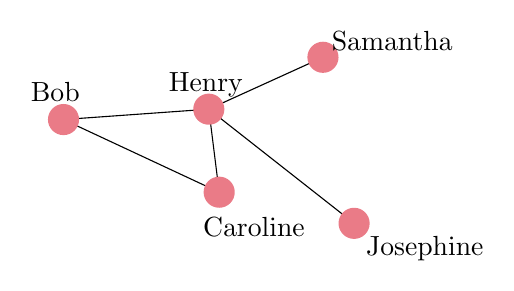
\begin{tikzpicture}[x=0.75pt,y=0.75pt,yscale=-.5,xscale=.5]
        %uncomment if require: \path (0,300); %set diagram left start at 0, and has height of 300
        %Straight Lines [id:da13877173221708183] 
        \draw    (155,125) -- (305,195) ;
        %Straight Lines [id:da4544026246030435] 
        \draw    (295,115) -- (405,65) ;
        %Straight Lines [id:da13798232124556553] 
        \draw    (295,115) -- (435,225) ;
        %Straight Lines [id:da570031360333461] 
        \draw    (295,115) -- (305,195) ;
        %Straight Lines [id:da7019239914549391] 
        \draw    (295,115) -- (155,125) ;
        %Shape: Circle [id:dp13093473233623887] 
        \draw  [draw opacity=0][fill={rgb, 255:red, 234; green, 123; blue, 135 }  ,fill opacity=1 ] (140,125) .. controls (140,116.72) and (146.72,110) .. (155,110) .. controls (163.28,110) and (170,116.72) .. (170,125) .. controls (170,133.28) and (163.28,140) .. (155,140) .. controls (146.72,140) and (140,133.28) .. (140,125) -- cycle ;
        %Shape: Circle [id:dp8544109743188051] 
        \draw  [draw opacity=0][fill={rgb, 255:red, 234; green, 123; blue, 135 }  ,fill opacity=1 ] (390,65) .. controls (390,56.72) and (396.72,50) .. (405,50) .. controls (413.28,50) and (420,56.72) .. (420,65) .. controls (420,73.28) and (413.28,80) .. (405,80) .. controls (396.72,80) and (390,73.28) .. (390,65) -- cycle ;
        %Shape: Circle [id:dp9935936256179412] 
        \draw  [draw opacity=0][fill={rgb, 255:red, 234; green, 123; blue, 135 }  ,fill opacity=1 ] (420,225) .. controls (420,216.72) and (426.72,210) .. (435,210) .. controls (443.28,210) and (450,216.72) .. (450,225) .. controls (450,233.28) and (443.28,240) .. (435,240) .. controls (426.72,240) and (420,233.28) .. (420,225) -- cycle ;
        %Shape: Circle [id:dp42474950398819455] 
        \draw  [draw opacity=0][fill={rgb, 255:red, 234; green, 123; blue, 135 }  ,fill opacity=1 ] (280,115) .. controls (280,106.72) and (286.72,100) .. (295,100) .. controls (303.28,100) and (310,106.72) .. (310,115) .. controls (310,123.28) and (303.28,130) .. (295,130) .. controls (286.72,130) and (280,123.28) .. (280,115) -- cycle ;
        %Shape: Circle [id:dp732541656718134] 
        \draw  [draw opacity=0][fill={rgb, 255:red, 234; green, 123; blue, 135 }  ,fill opacity=1 ] (290,195) .. controls (290,186.72) and (296.72,180) .. (305,180) .. controls (313.28,180) and (320,186.72) .. (320,195) .. controls (320,203.28) and (313.28,210) .. (305,210) .. controls (296.72,210) and (290,203.28) .. (290,195) -- cycle ;
        
        % Text Node
        \draw (121,87) node [anchor=north west][inner sep=0.75pt]   [align=left] {Bob};
        % Text Node
        \draw (411,37) node [anchor=north west][inner sep=0.75pt]   [align=left] {Samantha};
        % Text Node
        \draw (254,77) node [anchor=north west][inner sep=0.75pt]   [align=left] {Henry};
        % Text Node
        \draw (287,217) node [anchor=north west][inner sep=0.75pt]   [align=left] {Caroline};
        % Text Node
        \draw (444,235) node [anchor=north west][inner sep=0.75pt]   [align=left] {Josephine};
    \end{tikzpicture}
\end{document}